\documentclass[conference]{IEEEtran}
\IEEEoverridecommandlockouts
% The preceding line is only needed to identify funding in the first footnote. If that is unneeded, please comment it out.
\usepackage{cite}
\usepackage{amsmath,amssymb,amsfonts}
\usepackage{algorithmic}
\usepackage{graphicx}
\usepackage{textcomp}
\usepackage{xcolor}
\usepackage{url} 
\usepackage{listings}

\def\BibTeX{{\rm B\kern-.05em{\sc i\kern-.025em b}\kern-.08em
    T\kern-.1667em\lower.7ex\hbox{E}\kern-.125emX}}

\usepackage{xcolor}

\definecolor{codegreen}{rgb}{0,0.6,0}
\definecolor{codegray}{rgb}{0.5,0.5,0.5}
\definecolor{codepurple}{rgb}{0.58,0,0.82}
\definecolor{backcolour}{rgb}{0.95,0.95,0.92}

\lstdefinestyle{mystyle}{
    backgroundcolor=\color{backcolour},   
    commentstyle=\color{codegreen},
    keywordstyle=\color{magenta},
    numberstyle=\tiny\color{codegray},
    stringstyle=\color{codepurple},
    basicstyle=\ttfamily\footnotesize,
    breakatwhitespace=false,         
    breaklines=true,                 
    captionpos=b,                    
    keepspaces=true,                 
    numbers=left,                    
    numbersep=5pt,                  
    showspaces=false,                
    showstringspaces=false,
    showtabs=false,                  
    tabsize=2
}

\lstset{style=mystyle}

    
\begin{document}

\title{CS598 CCC Milestone 4\\
}

\author{
\IEEEauthorblockN{Cameron Greenwalt}
\IEEEauthorblockA{
\textit{UIUC}\\
Champaign, IL, USA \\
cg50@illinois.edu}
\and
\IEEEauthorblockN{Ming Meng}
\IEEEauthorblockA{
\textit{UIUC}\\
Champaign, IL, USA \\
mingm4@illinois.edu}
\and
\IEEEauthorblockN{Yang Peng}
\IEEEauthorblockA{
\textit{UIUC}\\
Champaign, IL, USA \\
yangp3@illinois.edu}
}
\maketitle


\section{Introduction and Project Idea}

AIOps, known as Artificial Intelligence for IT Operations, is a fairly recent development that focuses on applying machine learning to the IT Operations Space. AIOps is a new and exciting area within Cloud Computing and IT Operations. \cite{10212414, 10199929} Many major technology corporations such as IBM and Microsoft \cite{li2022an}  are actively conducting research in the area of AIOps. \cite{aiops-challenges} 

One of the biggest challenges in AIOps is that the cost and time for incorporating AI into the current IT Operations landscape is very expensive. It is often necessary to set-up a team of Machine Learning experts to train the models and understand its workflows. Therefore, we would like to minimize the use of training and finetuning steps by utilizing existing pre-trained Large Language Models (LLM) in the AIOps field.

LLMs have seen tremendous recent breakthroughs, especially in the generative AI space. ChatGPT, which uses OpenAI's GPT 3.5 LLM, was publicly released in late 2022 and had immediate major impacts in many fields. Much research in the industry has been focused on applying LLM and generative chatbots such as ChatGPT to different domains. 

We would like to use generative LLMs to summarize cloud application logs, thereby reducing the effort required for cloud engineers to perform tasks such as system maintenance and problem diagnosis. Existing research on logs in the AIOps space focuses more on log anomaly detection and classification tasks \cite{network-log-anomaly-detection}. Other common AIOps tasks include node failure prediction \cite{aiops-node-failures-alibaba}, CI/CD of ML apps \cite{mlops-ossara}, test case generation and bug detection \cite{model-checking-guided-testing}, task code generation \cite{mani2023enhancing}, incident management \cite{chen2020aiops, li2022an}, and documentation Q\&A/source code understanding \cite{source-code-understanding}. We will focus our research to the task of log summarisation using ChatGPT.


\section{Justification}
In this section, we present the justifications of the project idea. We believe that this project fulfills all three areas of Intellectual Merit, Novelty, and impact.

\subsection{Intellectual Merit}
Many natural language tasks in AIOps are done using models such as BERT \cite{network-log-anomaly-detection} that are fine-tuned using proprietary data or using rule-based approaches \cite{logrule}. The results with BERT, however, are dismal \cite{network-log-anomaly-detection} in many categories due to issues such as proprietary data availability for training, open source model limitations, and limited hardware acceleration resources. These challenges have hindered some of the development efforts in the AIOps field.

In this project, we will create embedding vectors from log data and use those as a basis of domain-specific knowledge for ChatGPT to tailor its generated log summary output. Prompts will be fed to ChatGPT in Azure cloud, which we believe is a good choice of cloud platform because it has a large market share and is secure.

\subsection{Novelty and Impact}
AIOps has been around for a while. However, as LLM technology is quite new and has only recently gained popularity due to the release of ChatGPT, most AIOps research still revolves around improving existing models/algorithms \cite{network-log-anomaly-detection}. Improving an existing model can be a very expensive operation due to the amount of GPU required for fine-tuning. Many businesses are unable to allocate the resources required to train a model from scratch. The use of traditional ML and DL techniques requires expert domain knowledge and expensive computational resources.

By using pre-trained state-of-art models from existing cloud providers and providing the models domain-specific or proprietary data, one can save computational resources and money by avoiding fine-tuning an existing model or training a model from scratch. This would be a more cost-effective way for businesses' IT teams to roll out AIOps solutions, which will in turn help the business' Site Reliability Engineers (SRE) more effectively address cloud incidents.

If our experiments yield good results, we believe that our work will have a great impact to the AIOps field and that many non-tech companies can apply our methods in small teams of engineers to monitor and improve a company's complex cloud infrastructure environment.

\section{Plan}
We will focus our efforts on the task of cloud log summarisation using generative LLMs.

We have identified some potential areas of difficulty we may encounter in this project:
\begin{itemize}
    \item Dataset selection
    \item Creating embeddings and storing them in Vector stores
    \item Integration with Azure AI Services
    \item Usability
    \item Achieving Good Results
\end{itemize}

For our dataset, we will use a sample set of Proxifier logs from the LogHub \cite{zhu2023loghub}.

We will use ChatGPT to generate our log summaries, as it is better-suited to this task than to other tasks such as anomaly detection and log classification.

\subsection{What system do you want to implement?}
Our system will be known as "A general AIOps framework on log data using LLM-generated results". The system involves a user passing sample log data to our prompt generator application, which will vectorize the provided logs and store them in a vector store. Then, users will submit a natural language query to the chatbot such as "Summarize this log for me: <log>". The chatbot then generates a prompt by utilizing the existing query embeddings from the vector store.

\begin{figure}[ht]
    \centering
    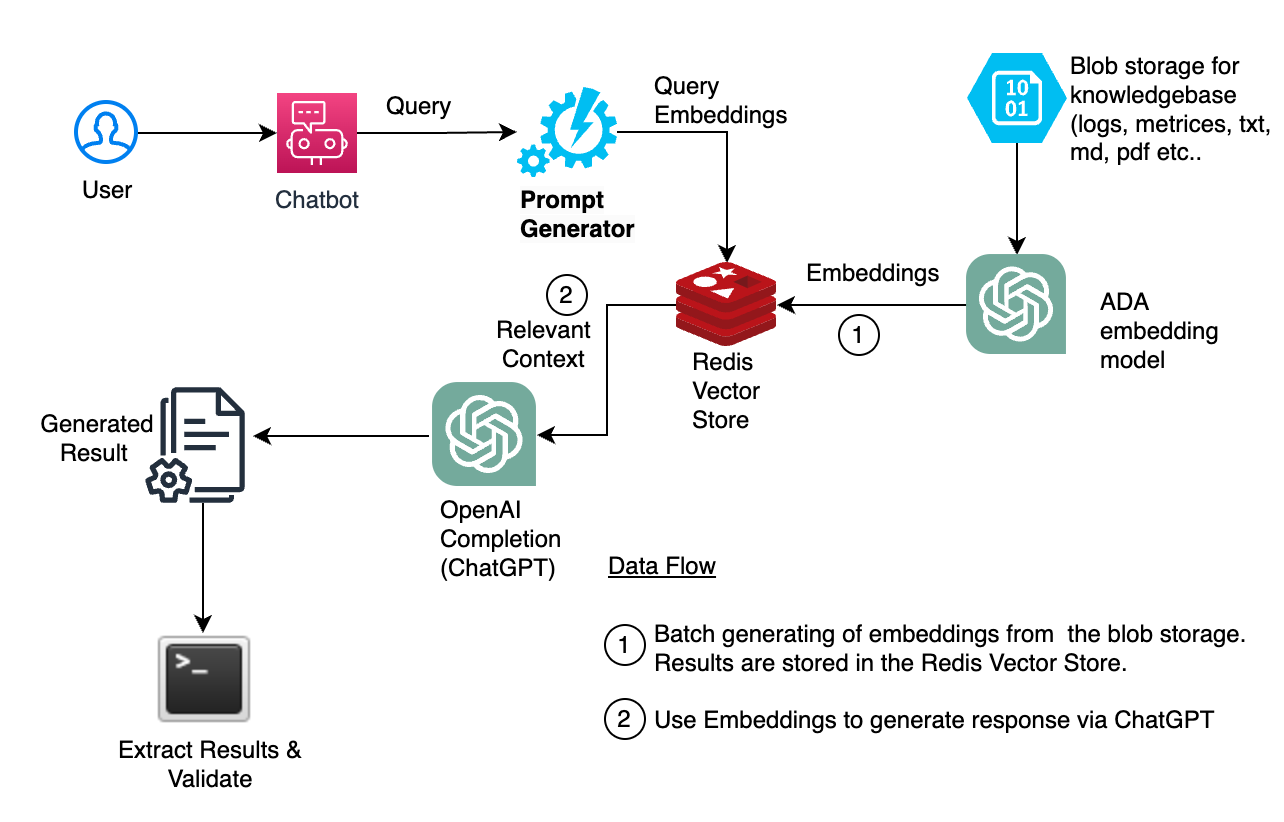
\includegraphics[width=0.4\textwidth]{arch.png}
    \caption{A proposed AIOps framework using LLM-generated results}
    \label{fig:arch}
\end{figure} 

Figure \ref{fig:arch} above shows the proposed implementation of the system. The chatbot can be either UI or API based. We plan to use Redis for the vector store, but another application such as Azure's Cloud AI vector store would work as well. The ADA embedding model will convert the provided data source into vector embeddings, which will be then be stored in the vector store. Then, the user submits a natural language prompt to our system. The prompt then becomes the input for ChatGPT. ChatGPT then uses the prompt, the log embeddings vector store, and its pretrained parameters to generate a summary of the log from the prompt. We will validate the generated result against a prelabeled result text file for accuracy. 


\section{THE EXPERIMENT- Modified for Milestone 3}

We divide our experiment into two categories: functional and infrastructure. The functional part describes how our system is going to function in terms of inputs and outputs. The infrastructure part describes the tools and services we will use to build our application.

\subsection{System to Build (Functional) - Modified for Milestone 3}

The system we are trying to build is using ChatGPT to summarize server logs from different applications. We believe that this would be very helpful for Site Reliability Engineers(SREs) for their day-to-day job for use-cases such as system maintenance and cloud incident response. By performing log summarisation tasks through the use of LLM, even non-subject-matter-experts can understand log output and therefore better understand software systems. Furthermore, management could also use the system to get a brief summary of the incident by feeding a few observed log lines to the prompt. The generated summary output could be used by the managers to provide better directions to the engineers. Overall, we envision that this system would improve efficiency, troubleshooting, and understanding.

We utilize the text embedding extracted from the documentation of vendors website and perform search embedding to generate queries with additional relevant contexts based on the user input, then feed them into ChatGPT to improve the log summary results. For example, when a user wants to know about the meaning from certain log extractions from a Proxifier server, it would go through a search embedding of Proxifier's official pdf documentation and do a cosine similarity search on the Redis vector database to generate a ChatGPT prompt with logs and additional related context related to the user input. We envision that the results shall be better than feeding a raw input from the user.


\subsection{System to Build (Infrastructure) - Modified for Milestone 3}

This section contains information from Figure 1 in our plan above. The main components in our system include the following:

\begin{enumerate}
    \item User- The users are mainly SREs or cloud engineers working on incidents. Management could also use this tool to obtain brief summary of an incident.
    \item Chatbot- This is the UI that the user will interact with.
    \item Prompt Generator- This is how the prompt will be generated, from matching the query embeddings stored in the Vector Stores.
    \item Data Source- The data source can be from various log sources within LogHub.
    \item Embedding data source- The embedding data source can be from various official or non-official documentation of the application.
    \item Embedding model- We are using ADA embedding model available in Azure Cloud.
    \item Vector Store - Redis Vector Store
    \item Output validation- Pre-labeled data-set, different metric scores, and/or manual validation.
\end{enumerate}

For our log data source, we will use logs from LogHub \cite{zhu2023loghub}, a public repository in GitHub that contains a collection of system/application logs. LogHub's log data are made freely accessible for AI-driven log analysis. The logs are not preproccessed in any way.

We will use logs from the Proxifier application as input to our model. Proxifier is a software that performs network proxy tasks. We chose to use Proxifier logs because the software is simple and the dataset is small enough for us to perform manual validation. Additionally, the Proxifier website has extensive documentation on how the software works.

\subsection{Hypothesis Tested - Modified for Milestone 3}\label{AA}

\textbf{Experiment Setting}
\begin{enumerate}
    \item Dataset: dataset is using logs provided by open source project\cite{liu2019logzip}. Each entry in the dataset provides row logs with a short summary. see the sample below for references.
    
    % See Figure \ref{fig:log} for more details.
    %     \begin{figure*}[ht]
    %     \centering
    %     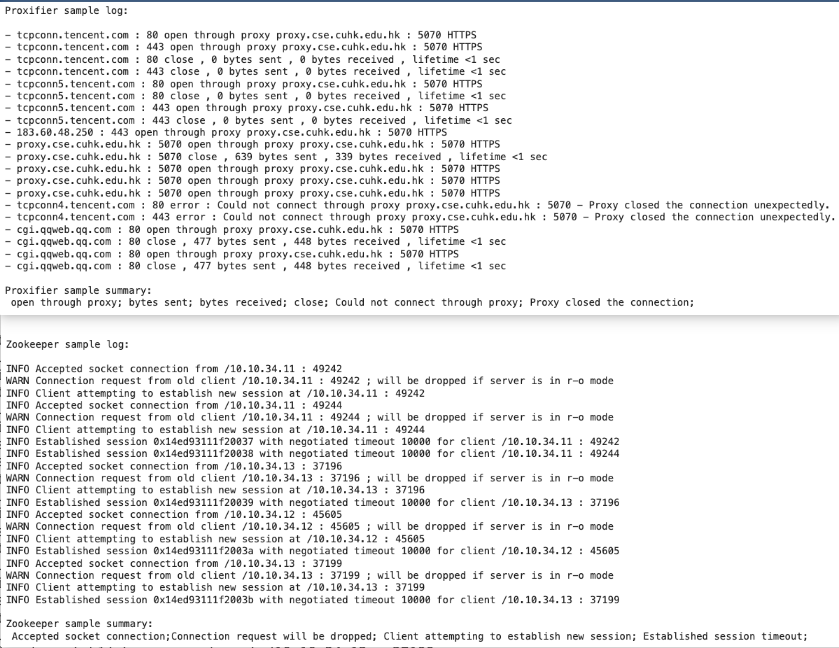
\includegraphics[width=\textwidth]{logs.png}
    %     \caption{sample log and summary}
    %     \label{fig:log}
    % \end{figure*} 
    \begin{lstlisting}[numbers=none]
# Proxifier sample log:

- tcpconn.tencent.com : 80 open through proxy proxy.cse.cuhk.edu.hk : 5070 HTTPS
- tcpconn.tencent.com : 443 open through proxy proxy.cse.cuhk.edu.hk : 5070 HTTPS
- tcpconn.tencent.com : 80 close , 0 bytes sent , 0 bytes received , lifetime <1 sec
- tcpconn.tencent.com : 443 close , 0 bytes sent , 0 bytes received , lifetime <1 sec
- tcpconn5.tencent.com : 80 open through proxy proxy.cse.cuhk.edu.hk : 5070 HTTPS
- tcpconn5.tencent.com : 80 close , 0 bytes sent , 0 bytes received , lifetime <1 sec
- tcpconn5.tencent.com : 443 open through proxy proxy.cse.cuhk.edu.hk : 5070 HTTPS
- tcpconn5.tencent.com : 443 close , 0 bytes sent , 0 bytes received , lifetime <1 sec
- 183.60.48.250 : 443 open through proxy proxy.cse.cuhk.edu.hk : 5070 HTTPS
- proxy.cse.cuhk.edu.hk : 5070 open through proxy proxy.cse.cuhk.edu.hk : 5070 HTTPS
- proxy.cse.cuhk.edu.hk : 5070 close , 639 bytes sent , 339 bytes received , lifetime <1 sec
- proxy.cse.cuhk.edu.hk : 5070 open through proxy proxy.cse.cuhk.edu.hk : 5070 HTTPS
- proxy.cse.cuhk.edu.hk : 5070 open through proxy proxy.cse.cuhk.edu.hk : 5070 HTTPS
- proxy.cse.cuhk.edu.hk : 5070 open through proxy proxy.cse.cuhk.edu.hk : 5070 HTTPS
- tcpconn4.tencent.com : 80 error : Could not connect through proxy proxy.cse.cuhk.edu.hk : 5070 - Proxy closed the connection unexpectedly.
- tcpconn4.tencent.com : 443 error : Could not connect through proxy proxy.cse.cuhk.edu.hk : 5070 - Proxy closed the connection unexpectedly.
- cgi.qqweb.qq.com : 80 open through proxy proxy.cse.cuhk.edu.hk : 5070 HTTPS
- cgi.qqweb.qq.com : 80 close , 477 bytes sent , 448 bytes received , lifetime <1 sec
- cgi.qqweb.qq.com : 80 open through proxy proxy.cse.cuhk.edu.hk : 5070 HTTPS
- cgi.qqweb.qq.com : 80 close , 477 bytes sent , 448 bytes received , lifetime <1 sec

# Proxifier sample summary:
 open through proxy; bytes sent; bytes received; close; Could not connect through proxy; Proxy closed the connection;


# Zookeeper sample log:

INFO Accepted socket connection from /10.10.34.11 : 49242
WARN Connection request from old client /10.10.34.11 : 49242 ; will be dropped if server is in r-o mode
INFO Client attempting to establish new session at /10.10.34.11 : 49242
INFO Accepted socket connection from /10.10.34.11 : 49244
WARN Connection request from old client /10.10.34.11 : 49244 ; will be dropped if server is in r-o mode
INFO Client attempting to establish new session at /10.10.34.11 : 49244
INFO Established session 0x14ed93111f20037 with negotiated timeout 10000 for client /10.10.34.11 : 49242
INFO Established session 0x14ed93111f20038 with negotiated timeout 10000 for client /10.10.34.11 : 49244
INFO Accepted socket connection from /10.10.34.13 : 37196
WARN Connection request from old client /10.10.34.13 : 37196 ; will be dropped if server is in r-o mode
INFO Client attempting to establish new session at /10.10.34.13 : 37196
INFO Established session 0x14ed93111f20039 with negotiated timeout 10000 for client /10.10.34.13 : 37196
INFO Accepted socket connection from /10.10.34.12 : 45605
WARN Connection request from old client /10.10.34.12 : 45605 ; will be dropped if server is in r-o mode
INFO Client attempting to establish new session at /10.10.34.12 : 45605
INFO Established session 0x14ed93111f2003a with negotiated timeout 10000 for client /10.10.34.12 : 45605
INFO Accepted socket connection from /10.10.34.13 : 37199
WARN Connection request from old client /10.10.34.13 : 37199 ; will be dropped if server is in r-o mode
INFO Client attempting to establish new session at /10.10.34.13 : 37199
INFO Established session 0x14ed93111f2003b with negotiated timeout 10000 for client /10.10.34.13 : 37199

# Zookeeper sample summary:
 Accepted socket connection;Connection request will be dropped; Client attempting to establish new session; Established session timeout;
 
\end{lstlisting}

      
    \item Embedding: The text embedding data-source is through the Proxifier official website. We downloaded the ProxifierWinV3.pdf from Proxifier's website and use it as our main source of text embedding.
    \item Setup: We will run our code on the Google Colab platform and use the Azure OpenAI service. The log summaries and embeddings are generated using the following models:
    \begin{itemize}
    \item gpt-35-turbo-16k
    \item gpt-4-32k
    \item text-embedding-ada-002
    \end{itemize}
    We picked 10 logs to process, as we are limited by the OpenAi throttling and processing capacity. 
    \item Evaluation: Once the summary is generated by calling the OpenAi services, we next calculate the lexical and semantic metrics to compare the quality of the generated text to the given summary.
\end{enumerate}

\textbf{Hypotheses - Modified for Milestone 3}

Below we propose 7 hypotheses/experiments to test. These experiments will test our application's ability to generate correct and readable summaries. We will incorporate the use of lexical and semantic scores to compare the relationships of the measurement outcomes.

\subsubsection{Our application should be able to handle text summarization}
\begin{itemize}
    \item \textbf{model}: gpt-4-32k or gpt-35-turbo-16k 
    \item \textbf{input}: sample logs
    \item \textbf{output}: log summarization
    \item \textbf{measurements}:
    \begin{itemize}
        \item correctness
        \item readability
        \item Lexical score, if possible
        \item Semantic score, if possible
    \end{itemize}
    \item \textbf{Zero-shot vs Few-shot}: 
 Zero-Shot and Few-Shot are the important capabilities of OpenAI's ChatGPT models. The test results shows Few-shot can generate more targeted and concise summary. In this case, we have generated a json payload which including keys like summary, throughput and anomaly. 
 we can also leverage few-shot to do the processing, for example, we re-format the log files to a more compacted templates by extracting the keywords. 
 
   \textbf{ Sample summary with zero-shot}
    \begin{itemize}
    \item baseline: 
    \begin{lstlisting}[numbers=none]
'open through proxy; bytes sent; bytes received; close;'
    \end{lstlisting}
    \item chatgpt3.5 summary: 
    \begin{lstlisting}[numbers=none]
The given content shows data about bytes sent and received, lifetime, and proxy connections.
    \end{lstlisting}
    \item chatgpt4 summary: 
    \begin{lstlisting}[numbers=none]
The proxy.cse.cuhk.edu.hk: 5070 has been closed and opened multiple times, with varying amounts of data sent and received.
    \end{lstlisting}
    \end{itemize}
    
   \textbf{ Sample summary with few-shot}
    \begin{itemize}
    \item proxifier log summary: 
    \begin{lstlisting}[numbers=none]
{
  "summary": "Multiple connections opened and closed through proxy.cse.cuhk.edu.hk with varying data transfer sizes.",
  "throughput": "Average throughput: 0.5 MB/s",
  "anomaly": "No anomalies detected."
}
{
"summary": "Multiple connections opened and closed via proxy, some with errors.",
"throughput": "Total sent: 1593 bytes, Total received: 1235 bytes",
"anomaly": "Unexpected proxy closure on tcpconn4.tencent.com"
}
\end{lstlisting}
It is impressive to see Chatgpt is able to calculate the throughput on the fly. however, the accuracy is a big concern as most of number it printed are not correct
\begin{lstlisting}[numbers=none]
{
  "summary": "Processed session terminations and expirations, accepted socket connection, warnings, and closed socket connection.",
  "anomaly": "None"
}
{"summary": "Multiple session terminations processed, some sessions expired due to timeout, one client connection closed.", 
"anomaly": "Old client connection request, end of stream exception caught."
}
\end{lstlisting}

    \end{itemize}

   \item  \textbf{Lexical Scores}

    \begin{figure*}[ht]
        \centering
        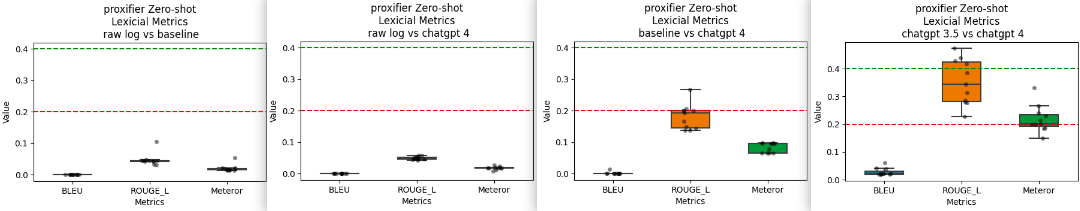
\includegraphics[width=\textwidth]{milestone4/proxifier_lexical_zero_shot.png}
       \caption{Proxifier Lexical metrics results with Zero-shot}        \label{fig:plz}
    \end{figure*} 
    
    Figure \ref{fig:plz} shows the proxifier summary lexical scores with zero-shot. The overall score seems low in general, but the content seems fine. The reference summary is very short and not totally human friendly. These characteristics of the reference summary may be the cause of the low lexical scores.
    
    \begin{figure*}[ht]
        \centering
        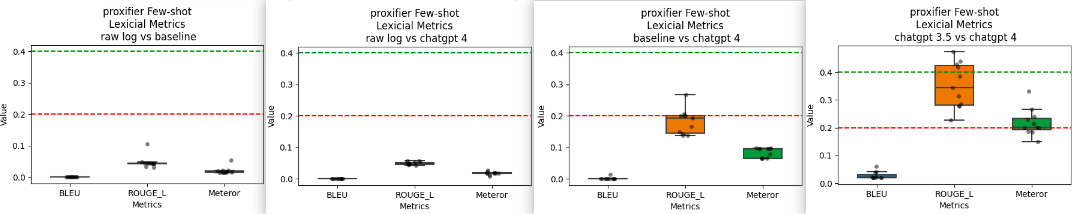
\includegraphics[width=\textwidth]{milestone4/proxifier_lexical_few_shot.png}
        \caption{Proxifier Lexical metrics results with Few-shot}
        \label{fig:plf}
    \end{figure*} 
    
    Figure \ref{fig:plf} shows the proxifier summary lexical scores with few-shot. it is pretty much the same level as the zero-shot
    

    \begin{figure*}[ht]
        \centering
        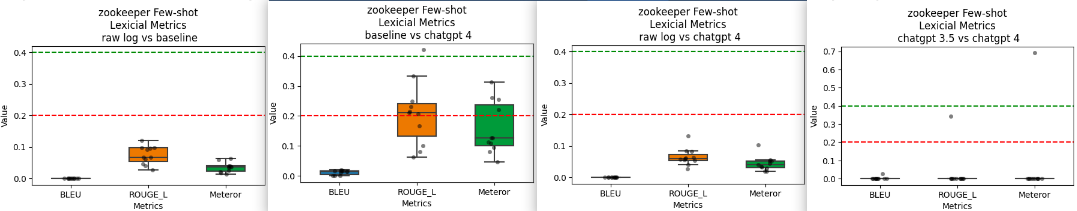
\includegraphics[width=\textwidth]{milestone4/zookeeper_lexical.png}
        \caption{ZooKeeper Lexical metrics results with Few-shot}
        \label{fig:zlf}
    \end{figure*} 
    
    Figure \ref{fig:zlf} shows the zookeeper summary lexical scores with few-shot. it is also low as general.

  As lexical score is mainly evaluating the vocabulary similarity, so it is not surprised to have the low lexical scores.
  
   \item \textbf{Semantic Scores}
    \begin{figure*}[ht]
        \centering
        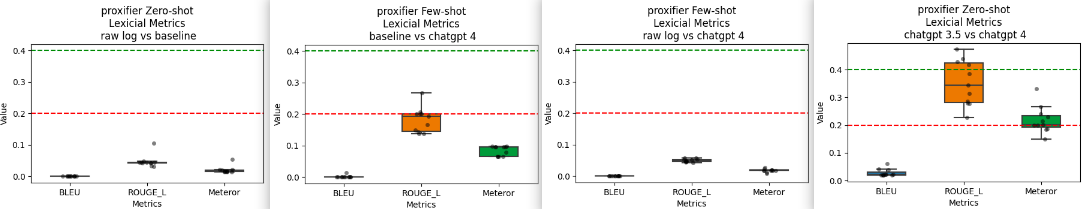
\includegraphics[width=\textwidth]{milestone4/proxifier_semantics_zero_shot.png}
        \caption{Proxifier Semantic metrics results with Zero-shot}
        \label{fig:psz}
    \end{figure*} 
    
    Figure \ref{fig:psz} shows the proxifier summary semantic scores with zero-shot. The overall score is slightly better. The score may have improved somewhat because the generated and reference summaries have some semantic similarity even though the actual vernacular is quite different.

    \begin{figure*}[ht]
        \centering
        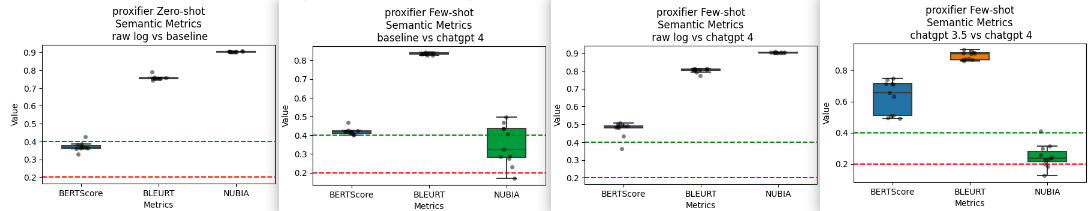
\includegraphics[width=\textwidth]{milestone4/proxifier_semantic_few_shot.png}
        \caption{Proxifier Semantic metrics results with Few-shot}
        \label{fig:psf}
    \end{figure*} 
        
    Figure \ref{fig:psf} shows the proxifier summary semantic scores with few-shot. The overall score is much better. The score shows it is benefits from the ChatGpts' Few-shot capability. It also shows the great potentials when using a proper prompt.

    \begin{figure*}[ht]
        \centering
        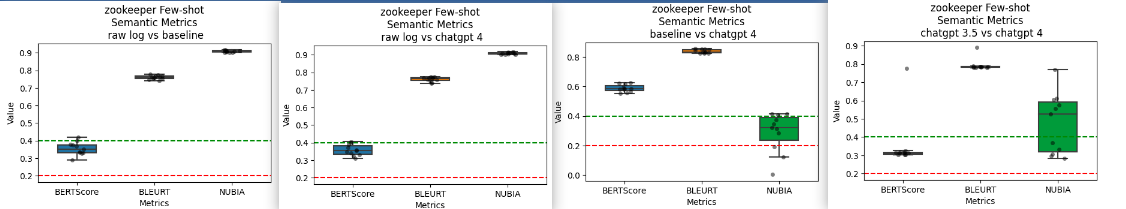
\includegraphics[width=\textwidth]{milestone4/zookeeper_semantics.png}
        \caption{ZooKeeper Semantic metrics results with Few-shot}
        \label{fig:zsf}
    \end{figure*} 

    Figure \ref{fig:zsf} shows the zookeeper summary semantic scores with few-shot. the number is consistent with the results from proxifier few-shot
    
    In general, ChatGPT summary seems verbose even when prompt hints to limit output are provided. We will need to conduct more tuning work. Some research has proposed an approach to use LoRA (Low-Rank Adaptation) to significantly reduces the number of trainable
    parameters\cite{hu2021lora}. If time permits, we can try incorporating that into our application.

 \end{itemize}
    

\subsubsection{Our application should be able to handle large text(over 100kb)}
\begin{itemize}
    \item \textbf{model}: gpt-4-32k or gpt-35-turbo-16k 
    \item \textbf{input}: sample logs
    \item \textbf{output}: log summarization
    \item \textbf{measurements}:
    \begin{itemize}
        \item correctness
        \item readability
        \item Lexical score if possible
        \item Semantic score if possible
    \end{itemize}
    \item \textbf{results}:
    As no surprises, both chatgpt3.5 and chatgpt 4 failed with the following error: 
    \begin{lstlisting}
    InvalidRequestError: This model's 
    maximum context length is 16384 
    tokens. However, your messages 
    resulted in 253056 tokens. 
    Please reduce the length of the 
    messages.
    \end{lstlisting}

    To work around this limitation, the first option is to feed the large input one chunk at a time, and then we can perform a summary of summaries. 
    
    As ChatGPT incorporates the use of memory networks to keep track of previous conversation and use the information to generate its responses, we expect that the feeding of input into ChatGPT in chunks will still satisfy our requirements.

    Some other AI services like Claude do not have size limitations. Claude can summarize multiple pdf documents. Regardless, we will limit our log input for this project. However, we should test out Claude's APIs if the limitation issue persists.
    
\end{itemize}


\subsubsection{Our application should be able to produce lexical score for a given text}
\begin{itemize}
    \item \textbf{input}: log summarization
    \item \textbf{output}: lexical score 
    \begin{itemize}
        \item human validation
    \end{itemize}
     \item \textbf{results}: 
     We will calculate the following metrics to determine lexical performance:
     \begin{itemize}
     \item BLEU
        \begin{itemize}
        \item Range from 0 to 1, Higher Is Better
        \item 0 indicates no in-betweenness similarity
        \item 1 indicates identical
        \item 0.4-0.6 is considered reasonable and 0.2-0.4 indicates some level of similarity
        \item above 0.6 is considered quite good
        \end{itemize}
    \item ROUGE
        \begin{itemize}
        \item Range from 0 to 1, Higher Is Better
        \item 0 indicates no in-betweenness similarity
        \item 1 indicates identical
        \item around 0.2-0.4 indicates some level of overlap
        \item above 0.4 is considered good
        \end{itemize}
    \item Meteor
        \begin{itemize}
        \item Range from 0 to 1, Higher Is Better
        \item 0 indicates no in-betweenness similarity
        \item 1 indicates identical
        \item 0.4-0.6 is considered reasonable and 0.2-0.4 indicates some level of similarity
        \item above 0.6 is considered quite good
        \end{itemize}
    \end{itemize}
\end{itemize}

\subsubsection{Our application should be able to produce a semantic score for a given text}
\begin{itemize}
    \item \textbf{input}: log summarization
    \item \textbf{output}: Semantic score 
    \item \textbf{measurements}:
    \begin{itemize}
        \item human validation
    \end{itemize}
 \item \textbf{results}: 
     We will calculate the following metrics to determine semantic performance:
    \begin{itemize}
    \item BERTScore \cite{bert-score}
        \begin{itemize} 
        \item range from 0 to 1, Higher Is Better
        \item 0 indicates no in-betweenness similarity
        \item 1 indicates identical
        \item 0.6-0.7 is considered good and indicates that the generated text is similar to the reference in terms of both vocabulary and context.
        \item above 0.6 is considered quite good
        \end{itemize}
    \item BLEURT \cite{bert-score}
        \begin{itemize}
        \item typically range from negative to positive
        \item A positive BLEURT score indicates that the generated text is considered better than randomly generated text. The higher the positive score, the better the quality.
        \item A negative BLEURT score suggests that the generated text is worse than randomly generated text. The lower the negative score, the worse the quality.
        \item A BLEURT score near zero implies that the quality of the generated text is neither better nor worse than randomly generated text.
        \end{itemize}
    \item NUBIA \cite{kane2020nubia}
        \begin{itemize}
        \item Range from 0 to 1, Higher Is Better
        \item Indicates how good of a substitute/replacement the candidate sentence is for the reference sentence.
        \end{itemize}
    \end{itemize}
\end{itemize}
\subsubsection{Our application should be able to create the embedding from the input logs}
\begin{itemize}
    \item \textbf{model}: ada
    \item \textbf{input}: sample logs
    \item \textbf{output}: log embedding
    \item \textbf{measurements}:
    \begin{itemize}
        \item human measurement
    \end{itemize}
    \item \textbf{results}: First, we extracted the official documentation from the Proxifier website. Then, we created embeddings using OpenAIEmbeddings through Azure OpenAI.
    \begin{itemize} 
    \item PDF Extraction: 
    We extracted the ProxifierWinV3.pdf file and fed that into the PyPDF2 pdf reader to read the documentation. Then we utilized Pandas to create a data-frame with two columns- Page Number and Page Text. We then read each page of the documentation sequentially and appended the page text to the dataframe. We validated that the number of pages in the dataframe matches that of the pdf.
    \item OpenAI Embeddings: 
    To create the embedding, we applied for access to Azure OpenAI and used the model "text-embedding-ada-002" to embed the data \cite{wang2023rethinking}. 
    \end{itemize}
    Overall, we were successful in creating the embeddings using a chunk size of 16.
\end{itemize}

\subsubsection{Our application should be able to store embeddings in the vector store}
\begin{itemize}
    \item \textbf{input}: embedding vector
    \item \textbf{output}: vector store
    \item \textbf{measurements}:
    \begin{itemize}
        \item embedding should be persistent
    \end{itemize}
    \item \textbf{results}: We stored the embeddings in the Redis vector store. We  validated that the results are stored successfully and are retrievable through our local client.
    \begin{itemize} 
    \item Redis Vector Store: First, we have to set-up redis-stack through Docker and expose it to a local docker network so our code running on Google Colab can connect to it. We have to digged through multiple tutorials online and have multiple test-and-try to set up. 
    \item Connect to Redis from Colab: We connect to Redis store using the redis library from Python, and test that we can store and retrieve a key-value pair to ensure connectivity and persistence of the store.
    \item Store Embedding into Redis Vector Store: We utilize the DataFrameLoader from LangChain and create a vectorstore through LangChain's RedisVectorStore method, with index as page number and the embedding created from Experiment 5. We validated the results were successful through redis-cli client running locally on our machine to ensure that we are able to get the embeddings which we just stored.
    \end{itemize}
\end{itemize}

\subsubsection{Our application should be able query embeddings from the vector store}
\begin{itemize}
    \item \textbf{input}: embedding input
    \item \textbf{output}: embedding output
    \item \textbf{measurements}:
    \begin{itemize}
        \item embedding should be searchable with a similarity score output
        \item relevant text output with page number
    \end{itemize}
    \item \textbf{results}
    To validate that the query embeddings work, we have to run some search queries manually taken from the ProxifierWinV3.pdf file. We randomly selected a few phrase and feed it to the query prompt, and use the vector store similarity function to obtain the top 10 search results with similarity scores.
\begin{figure}[h!]
    \centering
    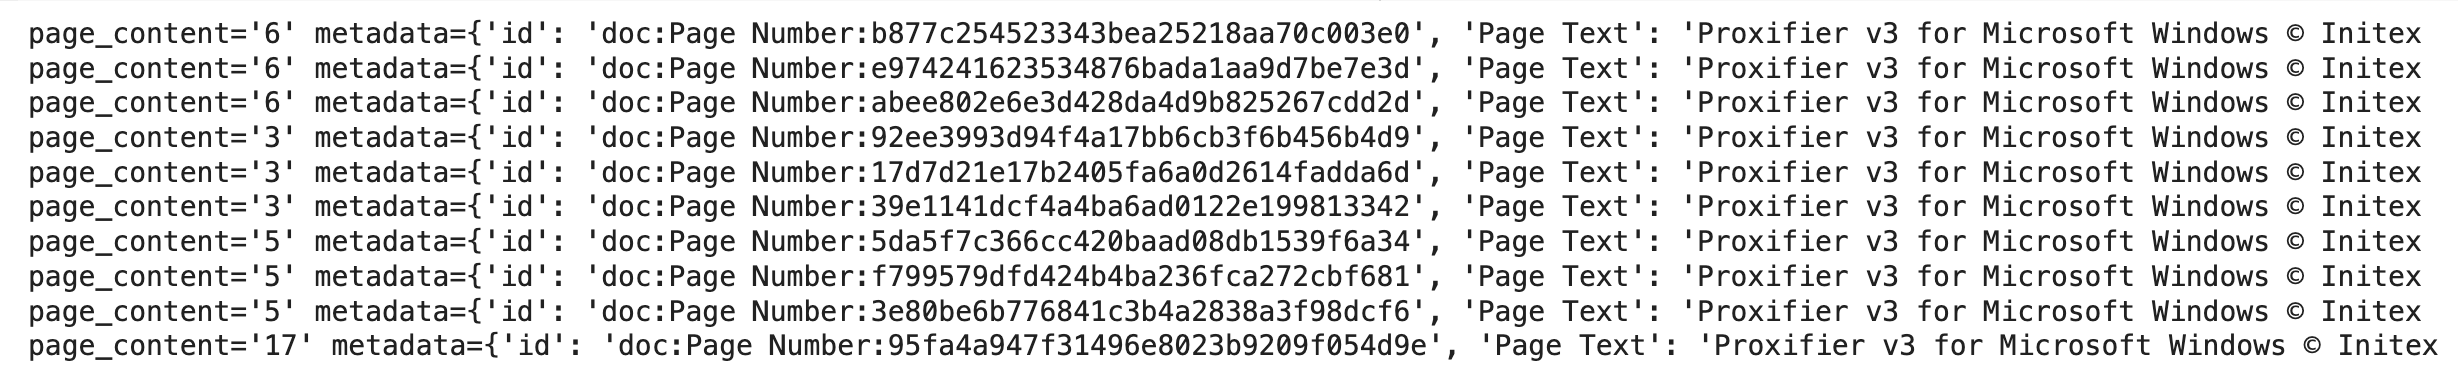
\includegraphics[width=0.5\textwidth]{pagenumber.png}
    \caption{Results with Page Number and Text}
    \label{fig:pagenumber-label}
\end{figure}
    
    Figure 5 shows the Search Results with Page Number. We successfully obtained top 10 Results and from a visual inspection the results appear to match certain keywords.
    
    The similarity score is computed from comparing the similarity between two vectors. We use it to determine the search performance:
    \begin{itemize}
        \item Similarity Score
        \begin{itemize}
            \item Range from 0 to 1, Higher Is Better
            \item 0 indicates there are no similarity between the two vectors
            \item 1 indicates that there is an exact match
            \item 0.4-0.6 is considered reasonable and 0.2-0.4 indicates some level of similarity.
            \item above 0.6 is considered quite similar
        \end{itemize}
    \end{itemize}
    The similarity score which we have obtained in our preliminary tests ranges from 0.25-0.26 range, indicates that the search yields with some level of similarity as from Figure 6 shown below. It is still far from ideal (0.6 or above) and our ultimate goal is to improve it at least close to the ideal range.
    We did not perform any type of section chunking, but rather through page chunk only. Some pagers may have more texts than others and may contain multiple sections. In addition, there are pages that contain information not quite useful for the prompt such as contacting customer support or the table of contents pages. We will try with different chunking methods and see which one actually yields a better similarity scores for our next Milestone. 
    \begin{figure} [h!]
        \centering
        \includegraphics[width=0.5\linewidth]{Similarity.png}
        \caption{Similarity Scores}
        \label{fig:similar-label}
    \end{figure}
\end{itemize}

\textbf{Hypotheses Validation Conclusions- Milestone 3}

Our hypothesis validation shows that there are still lots of refinements that can be tuned for text summary and search embeddings from the preliminary results. However, it is encouraging to see that the scores from our experiments did yield some non-zero scores with minimum of 0.2, which indicates some level of similarities. We will definitely need to experiment more with different types of prompts and search queries and we have some plans outlined in each of our 7 hypotheses above.

Note that in this Milestone experiments we have not combined our text embeddings with our prompt yet as we are still testing with Redis Vector store's similarity search capabilities, which is what we will be eventually combining to form our Prompt Generator. We plan to improve the similarity search scores and the lexical and semantic scores for log summarization first to be higher than reasonable range before writing our Prompt Generator.

A significant portion of our time during the Hypotheses Validation is actually spent on setting up the infrastructure for the experiments, and figuring out the correct libraries and tools to use from reading the tutorials online. Note that originally we plan to use the Cloud Vector store for text embeddings but eventually identified that it is too expensive to use, especially if we left it running for a longer time without deletion. Deleting it after each run is unsustainable and may waste lots of time. Therefore, we shifted the deployments to run on Google Colab but connect to the run-times locally, so that we can deploy the Redis Vector Database locally through Docker and connect from the Colab local runtime. 

\subsection{Measurements and Evaluation- Modified for Milestone 3}


We will use the ROUGE family of metrics in evaluating the performance of our log summaries. \cite{lin2004rouge} ROUGE metrics are a standard in the industry for text summarization evaluation. These metrics work by comparing a generated summary to a reference or "gold-standard" summary produced by a human. The dataset we plan to use in our research already includes human-created summaries for each log. We will use these preexisting, human-generated summaries as the standard for computing the ROUGE metrics.
We will also be comparing results of incorporating search embeddings vs raw search prompt to prove whether incorporating search embeddings into our Prompt Generator will yield better results.

We will also record several metrics relating to the performance of our system in the cloud such as latency of performing requests and running inferences, estimated cost of compute with Azure OpenAI, bandwidth limit, etc.

\subsection{Expected Successful Results}
We will compare the ROUGE F1 scores of our system to that of a very simple, no-ML baseline method \cite{medium-text-summarization} and to that of LogSummary. \cite{10017337} 

We will also perform qualitative analysis on our log summary. We understand that this step is subjective and may not come with a discrete metric, but we believe that human evaluation is beneficial in this case. It is important to evaluate the results manually as we need to ensure that the results are readable and make sense to our intended audiences such as SREs, developers, and managers.

% \section{Related Works- Modified for Milestone 3}
We have summarized our research from the previous milestones and divided into multiple sections for this milestone. It is extremely helpful to us in figuring out the steps to conduct our experiments and in drafting out our future plans.
\subsection{Log Summarization- Modified for Milestone 3}

LLMs offer an efficient and effective solution for many AIOps tasks. Common tasks include automated log analysis and log summarization, which enable SREs to address issues quickly and focus more resources on other mission critical tasks.\cite{gupta2023learning} Log summarization is useful because logs can contain complex, difficult to parse information that slows down diagnosis of cloud problems. Log summarization distills log data to a shorter, more natural-language friendly representation that can be quickly understood by cloud engineers.

While many previous research works have addressed the topic of log summarization, LogSummary \cite{10017337} is perhaps the work in closest relation to what we would like to accomplish in our research. LogSummary is an automatic and unsupervised log summarization framework that achieves an impressive ROUGE F1 score. The authors, upon finding that no"gold standard" labelled dataset of logs and their associated summaries exists, created their own dataset of logs and log summaries. They used this dataset to assess the quality of their models. We will use their opensource dataset in our work to assess the quality of our methods as well.

At the core of LogSummary is the LogIE algorithm, which "performs open information extraction on logs, extracting triples relating entities and arguments through relation or predicate." \cite{10017337} LogSummary does \textit{not} use generative LLMs such as ChatGPT, BERT, or derivatives. Rather, is uses a rule-based approach to extract information from logs. We plan to use LLMs to accomplish a similar objective while not being constrained to a particular output format or implementing a high-complexity system.

Some authors acknowledge that the ChatGPT model is more accurate than many other open source models that are presently available for summary generation. Additionally, ChatGPT often generates acceptable results without requiring a fine-tuning step prior to running inference. Presently, ChatGPT is the gold standard for most generative NLP tasks.\cite{bendimerad2023onpremise}

\subsection{Root Cause Analysis- Modified for Milestone 3}

Root cause analysis (RCA) is the task of diagnosing the causes for a cloud incident. The log data from relevant applications gathered during an incident is critical to diagnosing the root cause for the incident. Further, the rate at which a root cause for a cloud incident is identified can be accelerated by summarizing the related log data using AI.

LogRule \cite{logrule} is a Root Cause Analysis (RCA) algorithm, which, with a high F1-score of 0.921 and a 37x speed improvement over FP-growth, offers a time-efficient, accurate, and interpretable solution for RCA in complex datasets--especially where the current state-of-the-art algorithm struggles with execution times. LogRule aims to provide an explanation for specific events of interest, but it depends on structured rather than unstructured logs, which means that doing log preprocessing or overhauling a system's logs to all be structured would be prerequisites to using the system.

CloudRCA is "a root cause analysis framework for Alibaba Cloud's big data cloud computing platforms, utilizing heterogeneous multi-source data, state-of-the-art anomaly detection, and log analysis techniques to extract features, which are then employed in a Knowledge-informed Hierarchical Bayesian Network (KHBN) model." \cite{10.1145/3459637.3481903} CloudRCA is a thorough, useful system that is in-use in Alibaba's cloud systems and has provided a 20\% time savings for site reliability engineers (SREs). The cost for an organization to implement CloudRCA or a similar system in their own cloud platforms may exceed its relative benefit, and CloudRCA may not be applicable to somewhat dissimilar use cases. We envision that our work will have more general applicability and lower cost-to-implement for various organizations at the expense of narrower scope of operations (in this research, we will only perform log summarization).

In \cite{10172904}, researchers use LLMs in the following two scenarios:

1) Finding an incident's root cause. Diagnosing incidents typically requires significant time and communication before engineers can identify the root cause of the incident. Research showed that LLMs are effective at suggesting root causes for incidents.

2) Suggesting mitigation steps for incidents. After a root cause has been identified, engineers take actions to mitigate the problem. Research showed that LLMs are effective at recommending the mitigation steps for an incident.

\subsection{Comparison Models- Modified for Milestone 3}

BERT is a another very popular model used in natural language-based log tasks. Results with BERT are quite successful for very specific tasks such as detection and classification but suffer from a lack of generalizability to different problem scopes. In addition, tasks using BERT and its derivatives often require training and fine-tuning BERT for the specific task. This fine-tuning process can be time-consuming and expensive. \cite{LEE2023110689} In one research work, the authors used the RoBERTa model, which is a BERT derivative. The authors fine-tuned their model on both external and internal datasets, often borrowing popular new websites and articles. \cite{saha2022mining}

The performance of the anomaly log detection task using fine-tuned BERT-based models has proven to be very successful in recent research. For example, in one study, researchers were able to achieve an F1 score above 0.9 in detecting anomalies in a sample HDFS log dataset. This success can be attributed to the fact that HDFS log data has a simple log structure and has less natural language included in the logs. In fact, the authors found that pre-training BERT with more natural language data had a negative impact on anomaly detection. \cite{LEE2023110689} From these researchers' experience, we determined that LLMs are probably more suited for logs with more natural language semantics.

Another team of researchers used BERT-based models to build an intelligent-based system for IT Incident Operations. However, the metric scores they achieved with the base BERT models were quite low and often required other classifiers such as LSTMs to increase accuracy. The complexity of this system might lead to over-fitting issues. \cite{10189040} We would like our system to involve as little complexity as possible.

In assessing the viability of using GPT models for log- and cloud-related tasks, researchers at Microsoft studied over 40,000 incidents from 1000+ cloud services with six semantic and lexical metrics.\cite{10172904}  The following are the key insights from their work:
\begin{itemize}
    \item Fine-tuning significantly improves the effectiveness of LLMs for incident data.
    \item GPT-3 and GPT-3.5 models significantly outperform encoder-decoder models in our experiments.
    \item Metrics such as BLEU-4 are useful for measuring relative performance of models in different settings. However, manual inspection and validation with experts is required to assess actual performance.
\end{itemize}

Since we plan to emphasize the natural language characteristics of log data and model output and since we would like to keep the complexity of our system low, we will opt to use ChatGPT instead of BERT or other NLP models for the log summarization task. 

\subsection{Log Preprocessing- Modified for Milestone 3}

One area that we may find challenging in our research is in the log preprocessing step of the ML pipeline. We would like our proposed system to generalize to various log sources, but logs have a very diverse set of formatting rules and contexts. 

For example, logs are often found in semi-structured or, in many cases, unstructured formatting. There is no gold standard for logging specifications. Even top companies like Microsoft and Google have had issues with developing a systematic way to standardize logging practices among developers. This lack of log format standardization creates challenges in log parsing. Traditional methods will use regular expressions, keywords, grammar, algorithms, or even statistics to parse and read the logs. \cite{survey-log-aiops}

Most recent research in the area of log mining and parsing comes from the pre-ChatGPT era. For example, Logram is a library that uses traditional NLP methods such as leveraging n-gram dictionaries to achieve such tasks. \cite{10189040} The method of applying language models to log parsing and mining is still quite new. 

We may want to consider parsing/preprocessing logs using methods and software proposed previous research. For example, Drain+ \cite{10.1145/3540250.3558947} is a log parser that seeks to address the challenges of six other state-of-the-art log parsers. Drain+ outperforms the other parsers in a study of 16 public datasets.

Other popular ways of parsing logs include of clustering, pattern mining, and tree-based algorithms. LogMine and LogMa are two popular log parsing libraries that use log clustering with either a K-means algorithm or a hierarchical clustering algorithm. SLCT and LogCluster are two others that look for frequent log file items and perform pattern frequency-based mining. \cite{survey-log-aiops}

As logs from different applications and systems can be in various formats, it is important that we preprocess the log data to the intended formatting for our application. This means data transformation capabilities are required for our application's data injectors. One popular open-source tool used to ingest and process log data is Logstash, which is compliant with multiple databases/agents such as Telegraf. Alternatively, many proprietary software systems have their own data transformation capabilities that can be used to avoid having additional third-party dependencies. \cite{bendimerad2023onpremise}

\subsection{Prompt Generation- Modified for Milestone 3}

The performance of chat-based generative LLMs is heavily dependent on the correctness of the input prompts given to the model. When an incorrect or ill-posed prompt is used as input to ChatGPT, ChatGPT is likely to produce a poor output. The prompt needs to be carefully constructed and tuned to generate a specific output that matches the criteria of the user. Vector embeddings need to be used for example selection during the model's inference phase so that when the user issues a sample input, the system will match the input data to existing embeddings and automatically draft a prompt with relevant information to feed into ChatGPT. Note that logs can also contain non-text input and can exceed the input limit for many LLMs. These aspects will need to be considered in our research. For example, ChatGPT 3.5 has a 3000-word input limitation. \cite{zhoudb} To avoid ChatGPT input limit constraints, we plan to perform log summarization on an individual log basis. We have found that individual logs, from whatever application or datasource they may be from, generally do not contain more tokens than ChatGPT's input limit.

Below, we list some interesting tasks in the field of prompt engineering for LLMs:

\begin{itemize}
    \item improving the reasoning quality of LLMs through chain-of-thought and scratch-padding
    \item keeping LLMs self-consistent
    \item improving model results via multi-model debate
    \item verifying LLM responses
    \item teaching LLMs to use other tools
    \item retrieving relevant text from a large corpus, placing the text into context when needed
    \item providing a systematic architecture for tools to use LLMs
\end{itemize}

\subsection{Improving Model Performance- Modified for Milestone 3}

To improve model performance, LLMs can be fine-tuned with public and proprietary log data (transfer learning). Prior work processes multi-modal data (e.g., image, audio, text, etc.) with LLMs without explicit training. \cite{hamadanian2023a} 

Additionally, Some studies demonstrate that in order to improve task-agnostic, few-shot performance, scaling up the LLMs is often necessary. The GPT-3 model, which, when compared to many other language models, is itself a scaled up model, can achieve strong performance on many datasets. \cite{brown2020language} Other studies have explored how to generate a chain of thought, or a series of intermediate reasoning steps, that significantly improves the ability of LLMs to perform complex reasoning. \cite{wei2022chain}

The performance of LLMs in log related tasks can be improved by providing the models with more contextual data to use during inference. For example, log data can be used in conjunction with previous incident data to benefit incident management and resolution tasks. Automation can be performed with efficient ML models to generate diagnosis and resolution steps. This is especially powerful for urgent cases in which the assigned engineer can start diagnosing the issue and perform the suggested steps for resolution. However, performing this step requires past incident data which are often proprietary and can be difficult to obtain with existing publicly available datasets, especially when considering that the incident data has to correlate with the log data. \cite{bendimerad2023onpremise} 

Log data alone may not offer enough insights to produce high-quality generated responses from ChatGPT. Technical documentations, knowledge articles, and/or past incident investigations data can be used to provide contextual information to AIOps tasks, thereby improving task performance. Some examples of these kinds of data include a company's internal root cause knowledge source database, technical documentation of the application or related systems, troubleshooting guides, and software release notes. These data are often unstructured but are beneficial for the generation of analysis and summaries. \cite{saha2022mining}  In our research, we will provide ChatGPT with vector embeddings of the Proxifier documentation. We hypothesize that doing this will give ChatGPT more contextual information, thereby improving the quality of ChatGPT's generated summaries.

% \section{Summary}

Overall, we believe that our system is going to benefit companies of all sizes and improve their IT Operations workflows in a modern complex cloud infrastructure, as they often are unable to allocate the necessary resources and budget to train and fine-tune large ML models. We expect the following stakeholders to benefit from this project:
\begin{itemize}
    \item Site Reliability Engineers
    \item Platform Engineers 
    \item Management Audience 
    \item Incident Commanders 
\end{itemize}

We expect that SREs and Platform Engineers are the stakeholders that will benefit the most as our framework can used as an assistance tool for SREs when when maintaining cloud systems or responding to cloud incidents. Managers can use this tool to understand the current situation of the infrastructure without knowing many technical details. The incident commander can use this tool to ensure that the analysis is flowing in the right direction. Finally, we believe now is an optimal time to incorporate Generative AI into the corporate world within the IT Operations field. We hope this framework can transform how incident management, alerting, and root cause analysis are performed. 


\bibliographystyle{plain}
\bibliography{ref}
\vspace{12pt}

\end{document}
